\pagestyle{empty}
\vspace{18cm}
\begin{center}
\textbf{\Huge Capítulo 1}
\end{center}
\begin{center}
\textbf{\Huge Introdução ao Estudo}
\end{center}
\noindent\makebox[\linewidth]{\rule{\textwidth}{1pt}} 
\begin{flushleft}
Este capítulo visa abordar a seguinte questão de pesquisa:

Questão de pesquisa 1.1 - Que informações o corpo atual da literatura oferece a respeito do problema de pesquisa identificado?
\end{flushleft}
\noindent\makebox[\linewidth]{\rule{\textwidth}{1pt}} 

Este capítulo se encaixa nas etapas metodológicas a seguir:
\begin{figure}[ht]
\centering
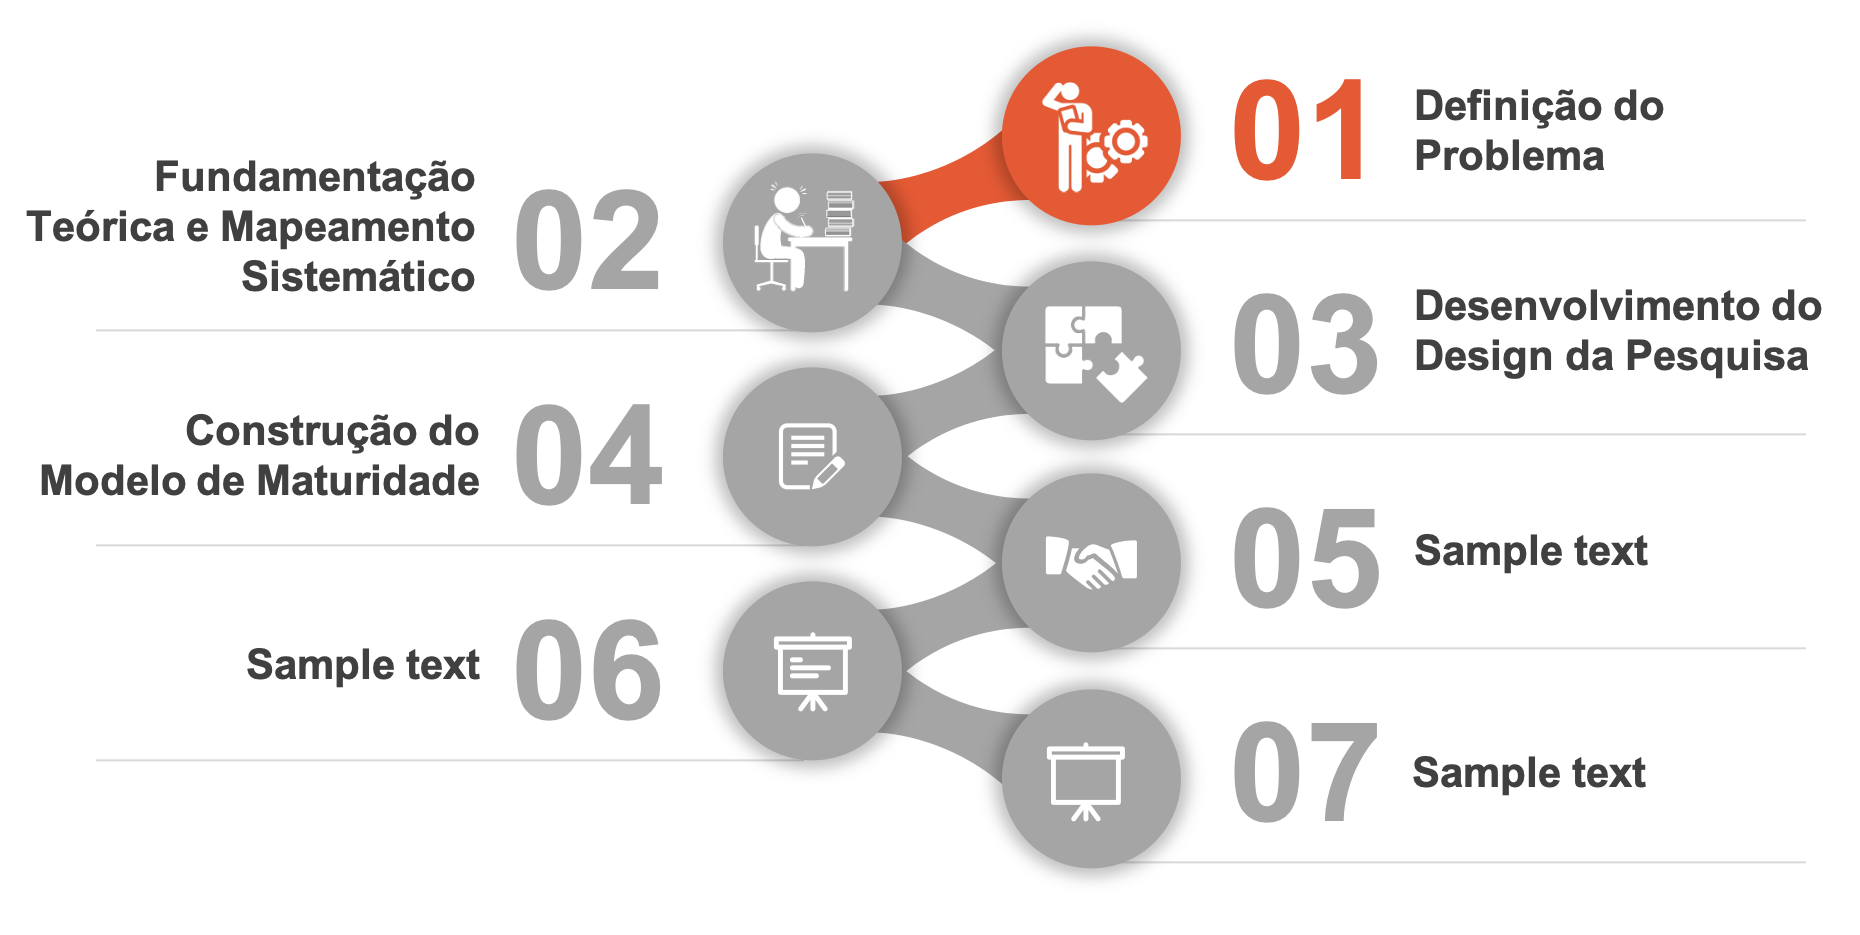
\includegraphics[width=15cm]{images/metodologia-cap1.png}
\label{fig:metodologia-cap1}
\end{figure}